% Preamble

\documentclass[a4paper,11pt,leqno]{article}
\usepackage[top=2.5cm, bottom=2.5cm, left=2.5cm, right=2.5cm]{geometry}	%Margins

\setcounter{tocdepth}{3}
\setcounter{secnumdepth}{3}
\renewcommand{\baselinestretch}{1.5} % Double spacing?

%\usepackage[framed]{mcode} %Matlab 
\usepackage{graphicx}        % standard LaTeX graphics tool

% Spaces in names of file locations

\usepackage[space]{grffile}

%My own

\usepackage{color}
\usepackage{amsmath}
\usepackage{hyperref}

\newcommand{\jk}[1]{{\color{blue}JK: #1}}

\newcommand{\ah}[1]{{\color{green}AH: #1}}



%% Equation numbering

\numberwithin{equation}{section}


\begin{document}


% Title bit

\title{Kickass document}
\author{Alice boo}

\maketitle

% Abstract

\begin{abstract}
This is the abstract.
\end{abstract}

% Table of contents

\tableofcontents

\newpage

\section{Introduction}

This thesis is structured as follows... It is long. In Section \ref{tissuelabel}, we do blabla. In particular, we compare our results with those in \cite{RN33}.

This equation is important:
%
$$e^{\pi i}+1=0,$$
%
where $\pi$ denotes that famous constant. And this other one I'm going to give a number to:
%
\begin{equation}\label{eq:anequation}
\int_0^\infty e^{-t}dt = 1.
\end{equation}
%
Then I can talk about Equation~\eqref{eq:anequation}. 

The color package allows you to write stuff in color, for example {\color{magenta} this in pink} and {\color{red} this in red}.

\subsection{Background theory}
%Here, I discuss some background.



Here, I talk about some background. I made some changes. Look at the cows in Figures \ref{fig:cow1}--\ref{fig:cow2}.

\begin{figure}[h]
	\begin{center}
	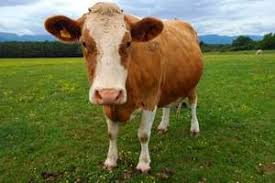
\includegraphics[width=0.45\textwidth]{./cowinside}
	\vspace{-20pt}
	\end{center}
\caption{\textbf{A splendid cow.} Look at this magnificent thing.}
\label{fig:cow1}
\end{figure}

More changes, cos I forgot something. Oh, here's a table, Table \ref{tab:table1}.

\begin{figure}
	\begin{center}
	\includegraphics[width=0.45\textwidth]{./cowoutside}
	\vspace{-20pt}
	\end{center}
\caption{\textbf{A splendid cow.} Look at this magnificent thing.}
\label{fig:cow2}
\end{figure}

\begin{table}[!ht]
\begin{center}
\begin{tabular}{c|cc|cccccccc}%\hline
$d$&$\leq4$&$5$&$6$&$7$&$8$&$9$&$10$&$11$&$12$&$13$\\     
\hline
$\rho_{x}^{d}$& $-\infty$   &  $0.4133$   &    $0.4134$  & $0.6202$ & $0.6202$   &$0.6365$    & $0.6365$   & $0.6376$ &$0.6377$&$0.6377$\\%\hline
$\eta_{x}^d$  &$\infty$   & $0.8283$   & $0.8282$  &   $0.6758$   & $0.6757$    & $0.6495$ &  $0.6495$&  $0.6494$&$0.6494$&$0.6428$ \\\hline
$d$&$14$&$15$&$16$&$17$&$18$&$19$&$20$&$21$&$22$&$23$\\\hline
$\rho_{x}^{d}$&$0.6377$&$0.6377$&$0.6377$&$0.6377$&$0.6377$&$0.6377$&$0.6377$&$0.6377$&$0.6377$&$0.6377$ \\
$\eta_{x}^d$  &$0.6428$ &$0.6404$&$0.6404$ &$0.6402$&$0.6402$&$0.6389$&$0.6389$&$0.6387$&$0.6387$&$0.6384$\\
\end{tabular}%}
\caption{Bounds on the mean of the stationary measures of the SDE~\eqref{eq:x3}. In total, $40$ bounds were computed taking a total CPU time of $10.3$ seconds, averaging $0.26$ seconds per bound.}
%\vspace{-20pt}
\label{tab:table1}
\end{center}
\end{table}

\section{Methods}

And bring up Equation~\eqref{eq:anequation} again. 


\subsection{Other stuff}

Another change. This final change convinces me.

\subsection{Tissue nonsense}\label{sec:tissuelabel}
This is how I do my shit.

\bibliographystyle{plain}

\bibliography{PhD_Endnote}

\end{document}